\documentclass{beamer}
\usetheme{Madrid}
\usecolortheme{whale}

\usepackage{amsmath,amssymb,amsfonts}
\usepackage{graphicx}

\title[75MW Solar Plant Integration]{Integration of 75MW Solar PV Plant:\\Transmission System Design Analysis}
\author{Brent Dickinson \and Tianci Xie}
\date{December 10, 2024}

\begin{document}
	
	\begin{frame}
		\titlepage
	\end{frame}
	
	\begin{frame}{Project Objectives}
		Design transmission system modifications to:
		\begin{itemize}
			\item Integrate 75 MW solar PV at NEWSOLAR substation
			\item Provide redundant transmission paths
			\item Resolve existing system violations
			\item Maintain stability under N-1 contingency
			\item Minimize total cost including 5-year loss reduction
		\end{itemize}
	\end{frame}
	
	\begin{frame}{Initial System Analysis}
		\begin{columns}[T]
			\begin{column}{0.4\textwidth}
				Base System Characteristics:
				\begin{itemize}
					\item Total load: 826.3 MW, 275.5 Mvar
					\item Generation: 837.7 MW from 10 generators
					\item System losses: 10.7 MW (1.3\%)
					\item Reactive support: -122.5 Mvar from 9 switched shunts
				\end{itemize}
			\end{column}
			\begin{column}{0.6\textwidth}
				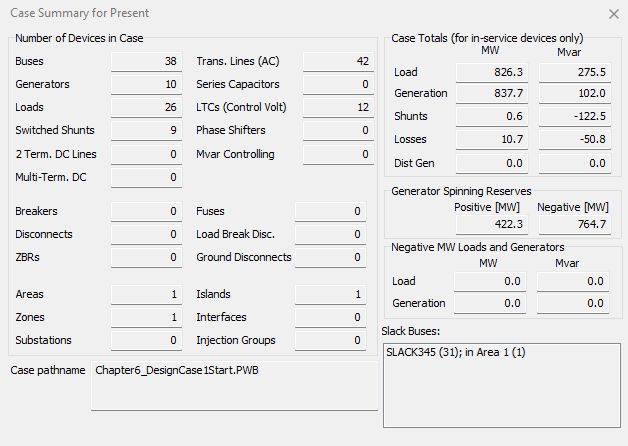
\includegraphics[width=1\linewidth]{figures/case_summary_existing}
			\end{column}
		\end{columns}
	\end{frame}
	
	\begin{frame}{Existing System Violations}
		\begin{table}
			\centering
			\begin{tabular}{|l|c|c|c|}
				\hline
				\textbf{Contingency} & \textbf{Flow} & \textbf{Limit} & \textbf{\%} \\
				\hline
				\textit{PINE138-PINE69 Xfmr:} & & & \\
				OAK69-BUCKEYE69 & 760.3 & 686.1 & 110.8 \\
				BUCKEYE69-APPLE69 & 454.2 & 418.4 & 108.6 \\
				\hline
			\end{tabular}
		\end{table}
		\centering
		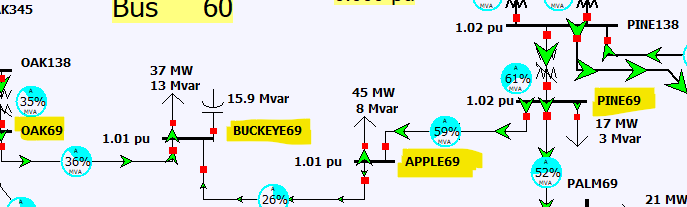
\includegraphics[width=0.7\linewidth]{figures/base_violations}
	\end{frame}
	
	\begin{frame}{Design Approach}
		\begin{itemize}
			\item Evaluate all possible connection configurations
			\item Compare 69 kV vs 138 kV options
			\item Start with shortest distance solution
			\item Use least expensive conductors initially
			\item Upgrade components only as needed
			\item Consider loss reduction benefits
		\end{itemize}
	\end{frame}
	
	\begin{frame}{Candidate Solutions}
		19 possible configurations evaluated:
		\begin{itemize}
			\item 69 kV options: \$5.94M - \$12.23M
			\item 138 kV options: \$14.37M - \$19.42M
			\item Shortest path: NEWSOLAR to BUCKEYE69 \& APPLE69 (12 km)
			\item Required upgrade: OAK69-BUCKEYE69 to Crow conductor
		\end{itemize}
	\end{frame}
	
	\begin{frame}{Selected Solution Cost Breakdown}
		\begin{table}
			\centering
			\begin{tabular}{|l|r|}
				\hline
				\textbf{Component} & \textbf{Cost (M\$)} \\
				\hline
				OAK-BUCKEYE Upgrade & 3.87 \\
				NEWSOLAR-BUCKEYE Line & 2.97 \\
				NEWSOLAR-APPLE Line & 2.97 \\
				Loss Savings (0.9 MW) & -2.37 \\
				\hline
				\textbf{Total} & \textbf{7.44} \\
				\hline
			\end{tabular}
		\end{table}
	\end{frame}
	
	\begin{frame}{Loss Reduction Analysis}
		\begin{columns}[T]
			\begin{column}{0.4\textwidth}
				\begin{itemize}
					\item Base case losses: 10.7 MW
					\item New configuration: 9.8 MW
					\item Savings: 0.9 MW
					\item 5-year energy savings: 39,420 MWh
					\item Economic value: \$2.37M at \$60/MWh
				\end{itemize}
			\end{column}
			\begin{column}{0.6\textwidth}
				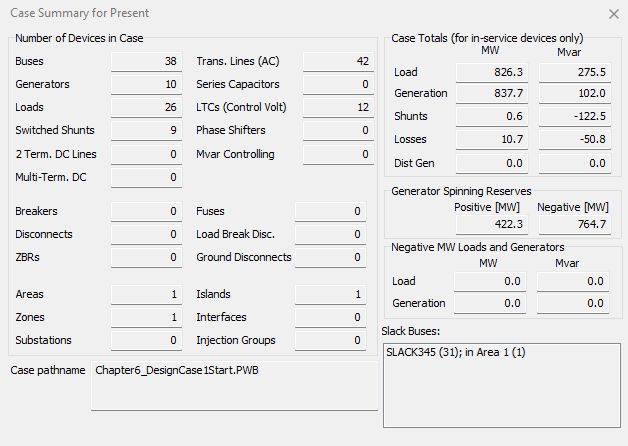
\includegraphics[width=1\linewidth]{figures/case_summary_existing}
			\end{column}
		\end{columns}
	\end{frame}
	
	\begin{frame}{Conclusions}
		\begin{itemize}
			\item Optimal solution: 69 kV connections to BUCKEYE \& APPLE
			\item OAK-BUCKEYE upgrade resolves contingency violations
			\item Total cost \$7.44M including loss savings
			\item Meets all reliability and redundancy requirements
			\item Simple design facilitates implementation
		\end{itemize}
	\end{frame}
	
	\begin{frame}{Questions?}
		\centering
		\Large{Thank you!!}
	\end{frame}
	
\end{document}